\documentclass{article}

\usepackage{graphicx}
\usepackage{tikz}
\usepackage{tikzsymbols}
\usetikzlibrary{calc,patterns,shapes.geometric}
\pagestyle{empty}
\usepackage[margin=0pt]{geometry}
\geometry{papersize={14in,12in}}

\def\centerarc[#1](#2)(#3:#4:#5){\draw[#1] ($(#2)+({#5*cos(#3)},{#5*sin(#3)})$) arc (#3:#4:#5);}

\begin{document}
	\begin{figure}
		\centering
		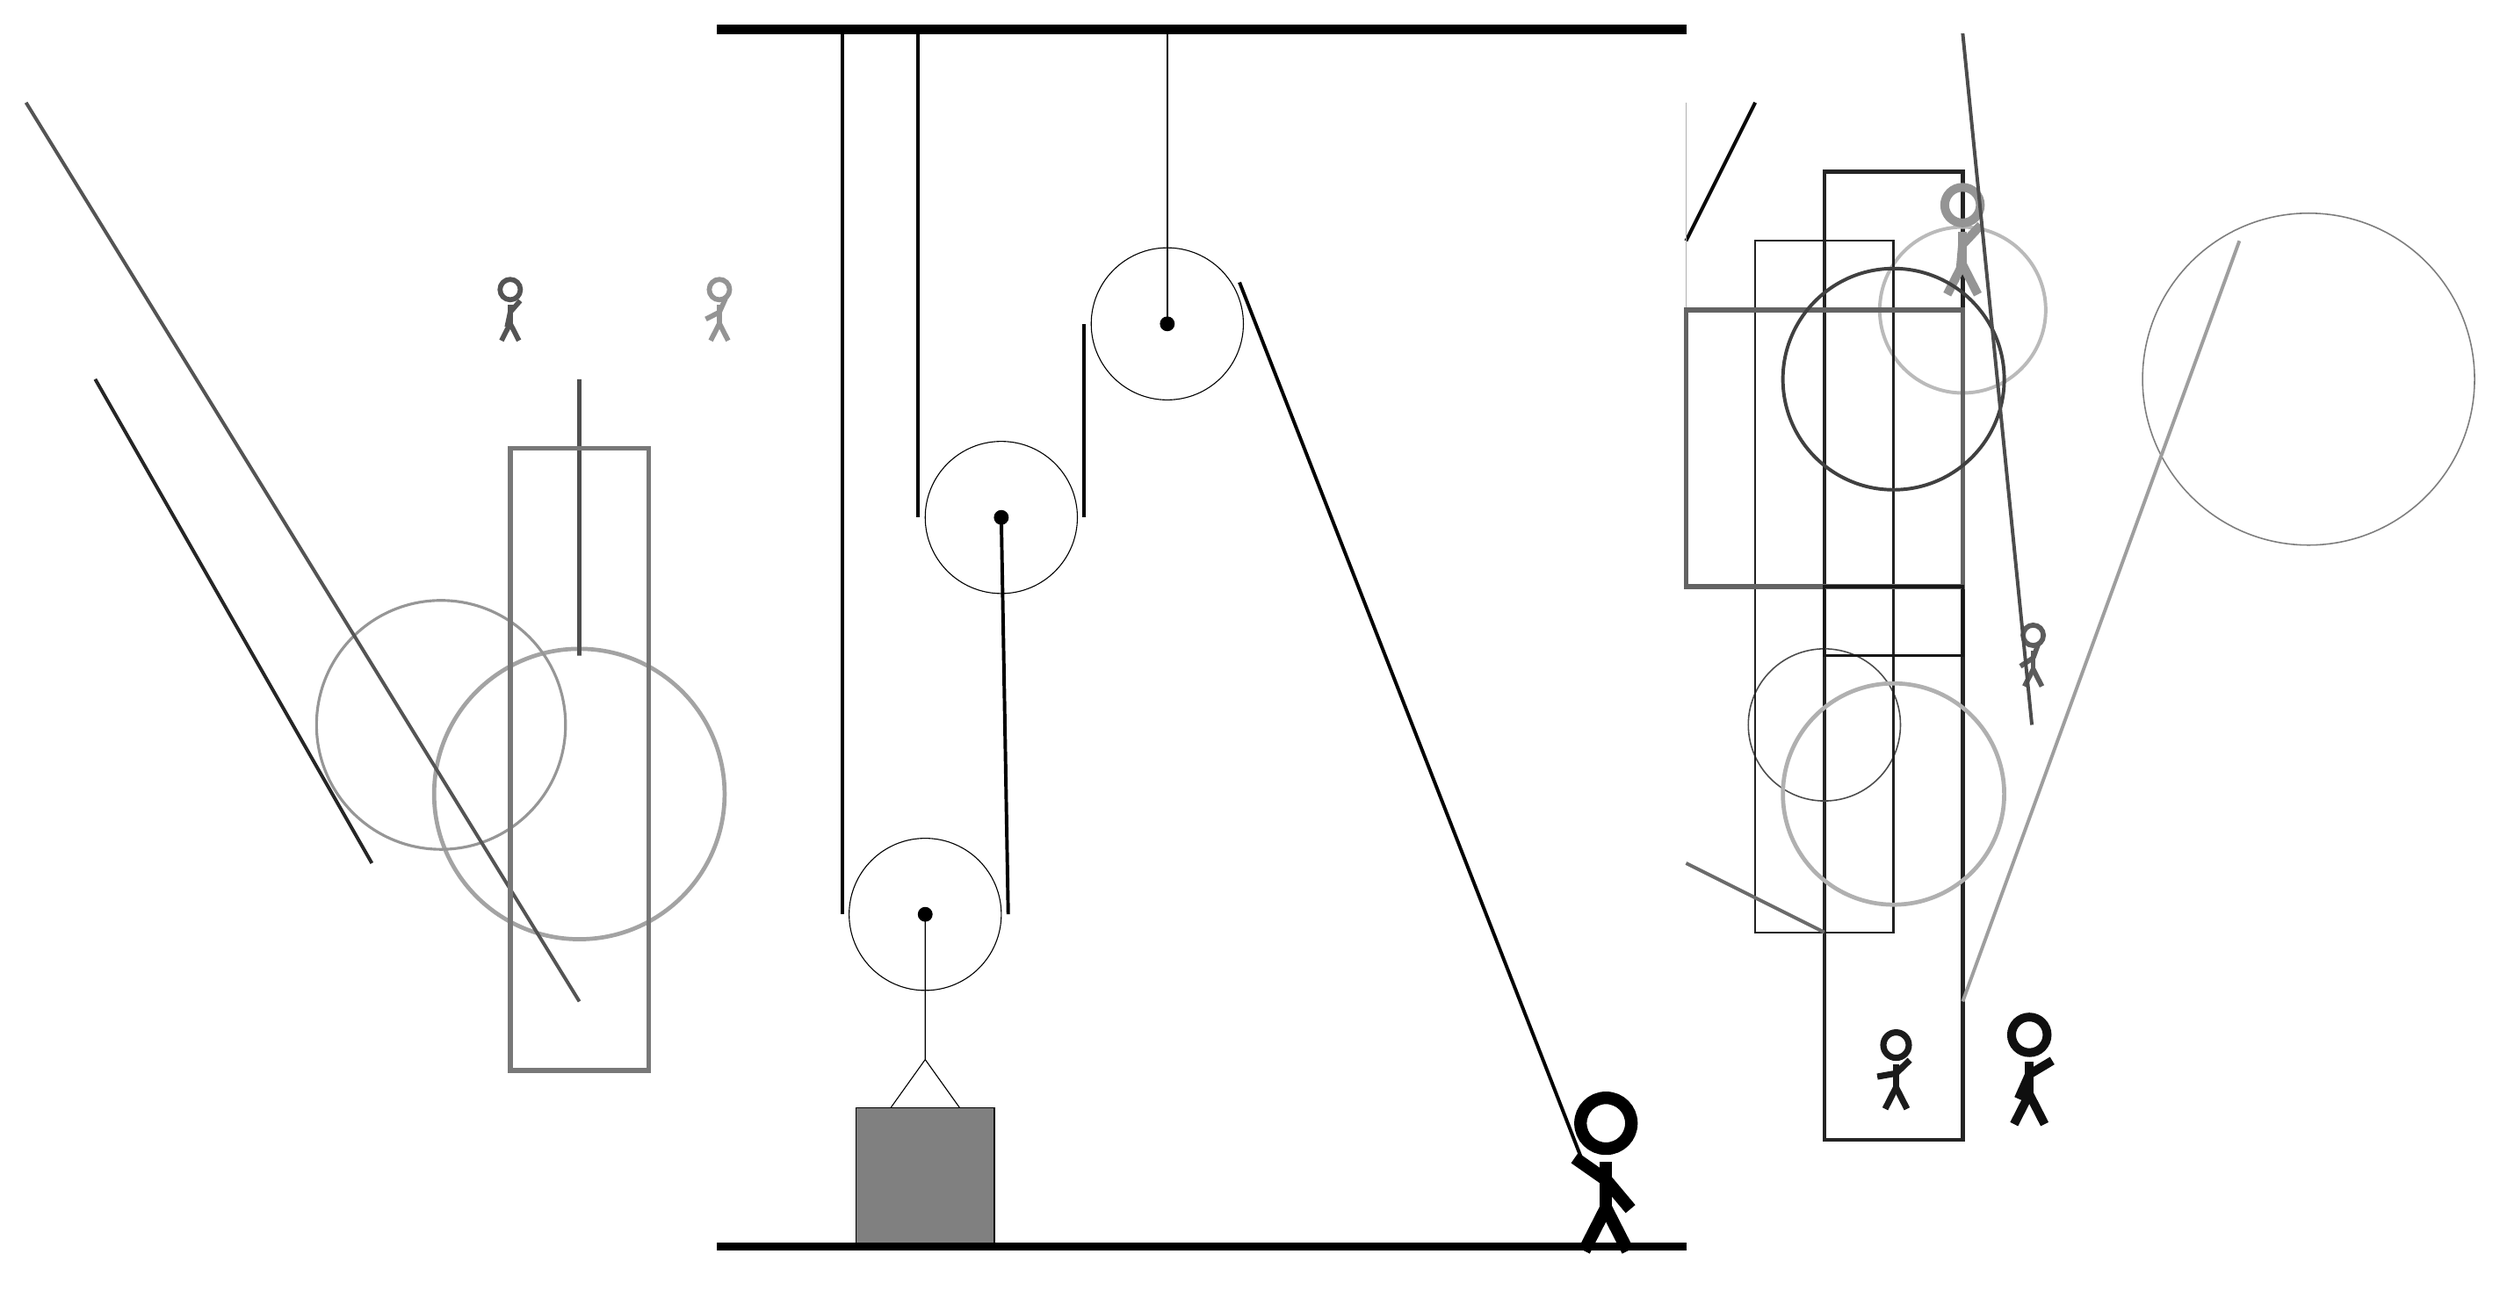
\begin{tikzpicture}
			%%%%% START %%%%%
			
			\draw[fill=black] (-2, 14) rectangle (12, 14.125);
			
			\draw (1, 1.26) circle (1.1);
			\draw[fill=black] (1, 1.26) circle (0.1);
			
			\draw (2.1, 7.0) circle (1.1);
			\draw[fill=black] (2.1, 7.0) circle (0.1);
			
			\draw[line width=0.5mm, color=black!97](12, 11) -- (13, 13);
			
			\node[line width=0.2mm, color=black!64] at (17, 5) {\Strichmaxerl[4][33][70]};
			\draw [line width=0.6mm, color=black!36](-4, 3) circle (2.1);
			\draw[line width=0.6mm, color=black!86] (14, -2) rectangle (16, 12);
			
			\node[line width=0.7mm, color=black!94] at (17, -1) {\Strichmaxerl[7][66][31]};
			\draw [line width=0.2mm, color=black!70](14, 4) circle (1.1);
			\draw [line width=0.5mm, color=black!27](16, 10) circle (1.2);
			\draw [line width=0.4mm, color=black!41](-6, 4) circle (1.8);
			\node[line width=0.4mm, color=black!89] at (15, -1) {\Strichmaxerl[5][10][44]};
			\node[line width=0.5mm, color=black!42] at (-2, 10) {\Strichmaxerl[4][27][66]};
			\draw[line width=0.3mm, color=black!87] (13, 11) rectangle (15, 1);
			\node[line width=0.4mm, color=black!42] at (16, 11) {\Strichmaxerl[7][85][47]};
			\draw[line width=0.5mm, color=black!67](-4, 0) -- (-12, 13);
			
			\draw[line width=0.2mm, color=black!31] (12, 10) rectangle (12, 13);
			\draw[line width=0.5mm, color=black!58](12, 2) -- (14, 1);
			\draw[line width=0.7mm, color=black!61] (12, 10) rectangle (16, 6);
			\node[line width=0.6mm, color=black!67] at (-5, 10) {\Strichmaxerl[4][78][49]};
			
			\draw[line width=0.6mm, color=black!69] (-4, 9) rectangle (-4, 5);
			\draw [line width=0.5mm, color=black!75](15, 9) circle (1.6);
			\draw[line width=0.5mm, color=black!70](16, 14) -- (17, 4);
			\draw[line width=0.7mm, color=black!53] (-3, -1) rectangle (-5, 8);
			
			\draw [line width=0.6mm, color=black!31](15, 3) circle (1.6);
			\draw [line width=0.2mm, color=black!51](21, 9) circle (2.4);
			\draw[line width=0.4mm, color=black!91] (14, 5) rectangle (16, 6);
			\draw[line width=0.5mm, color=black!38](16, 0) -- (20, 11);
			
			\draw[line width=0.5mm, color=black!85](-7, 2) -- (-11, 9);
			
			\draw (4.5, 9.8) circle (1.1);
			\draw[fill=black] (4.5, 9.8) circle (0.1);
			\draw[thick] (4.5, 9.8) -- (4.5, 14);
			
			\draw (1, 1.26) -- (1, -0.84) -- (0.5, -1.54) -- (1.5, -1.54) -- (1, -0.84);
			\draw[fill=black!50] (0, -1.54) rectangle (2, -3.54);
			
			\draw[line width=0.5mm] (-0.2, 14) -- (-0.2, 1.26);
			\centerarc[line width=0.5mm](1, 1.26)(180:360:1.2000000000000002);
			\draw[line width=0.5mm](2.2, 1.26) -- (2.1, 7.0);
			\draw[line width=0.5mm] (0.9, 14) -- (0.9, 7.0);
			\centerarc[line width=0.5mm](2.1, 7.0)(180:360:1.2000000000000002);
			\draw[line width=0.5mm](3.3, 7.0) -- (3.3, 9.8);
			\centerarc[line width=0.5mm](4.5, 9.8)(30:180:1.2000000000000002);
			\draw[line width=0.5mm] (5.544, 10.4) -- (10.5, -2.3);
			
			\node at (10.8, -2.5) {\Strichmaxerl[10][-35][-50]};
			
			\draw[fill=black] (-2, -3.5) rectangle (12, -3.6);
			
			%%%%% END %%%%%
		\end{tikzpicture}
	\end{figure}	
\end{document}